\chapter{DaVid} \label{cha:DaVid}

In diesem Kapitel werden das DaVid System beschrieben. Zuerst läuft die Vorstellung des DaVid-Systems. Die Systemmodell und Arbeitsprinzip des Systems werden in anschließenden Abschnitt erläutert. Schließlich folgt die mögliche Anwendungsgebiete des Systems.
%Durch diese Beschreibung wird die Bedeutung und Ziele dieses Papiers besser verstehen.\ldots

\section{Einführung des DaVids} 

DaVid, abkürzt von \uline{Da}ta transmission using \uline{Vi}deo \uline{d}evices, ist ein neuartiges Verfahren zur optischen Freiraum-Datenübertragung zwischen einem Display als Sender und einer Kamera als Empfänger. Ein grundlegendes Übertragungskonzept von DaVid wird in Abbildung 2.1 gezeigt. Ein flaches Display wie ein OLED- oder LCD-Bildschirm zeigt ein Live-Video. Gleichzeitig werden die Daten hinter dem Bild auf die Pixel moduliert. Während die zusätzliche Datenmodulation für menschliche Betrachter nahezu unsichtbar ist, der Benutzer leitet ein hochauflösende Kamera oder ein Smartphone zur Bildschirm, um die Szene aufzunehmen. Durch der eingebaut Prozessor können die Signale decodiert werden.

\begin{figure}[htb]
 \centering 
 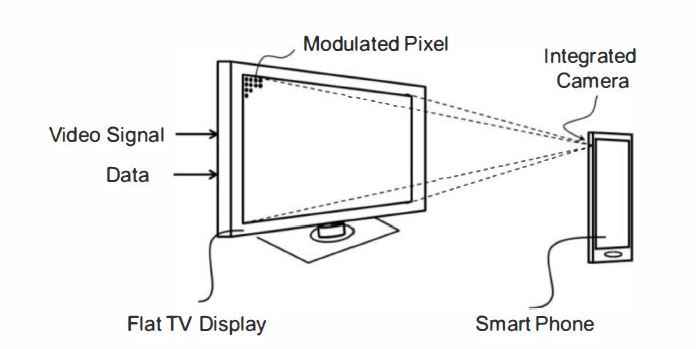
\includegraphics[keepaspectratio,width=0.8\textwidth]{images/David1.jpg}
 \caption{Eine beispielhafte Implementierung des DaViD-Systems}
 \label{fig:David1}
\end{figure}


\section{Systemmodell} 
Bild in Display enthalten eine große Anzahl von Pixeln, die jeweils aus einer spezifischen Anordnung von Subpixeln für die RGB-Farbraum bestehen. Jeder einzelne Frame des Videos wird nämlich durch eine Matrix von Subpixelwerten dargestellt. DaVid System verwendet eine differentielle Modulationsmethod d.h. Teil der Videoinformationen muss wiederholt werden, indem Daten als ein symmetrischer Manchester-Code moduliert und zu den Videosignalkomponenten hinzugefügt werden. In Empfängerseite durch eine zeitliche Synchronisation können die zeitliche \gls{ISI} vermieden werden. Dann nach Verwendung einer örtlichen Synchronisation enthalten einen Differenzbild. Weil die Randbereich des Differenzbilds ungültig ist, verlässt sich die Modulationsgebiet durch die Verfahren in diese Arbeit entdecken. Danach werden die überlagerten Datensequenz durch eine Reihe von Behandlungen vom Videoinhalt getrennt. Abbildung 2.2 zeigt die schematische Darstellung des DaVid-Systems. 
% Deshalb in zeitlicher oder örtlicher Richtung die Videoinhalt in paar Bildern werden gleich.
\vspace{18pt}

\begin{figure}[htb]
	\centering 
	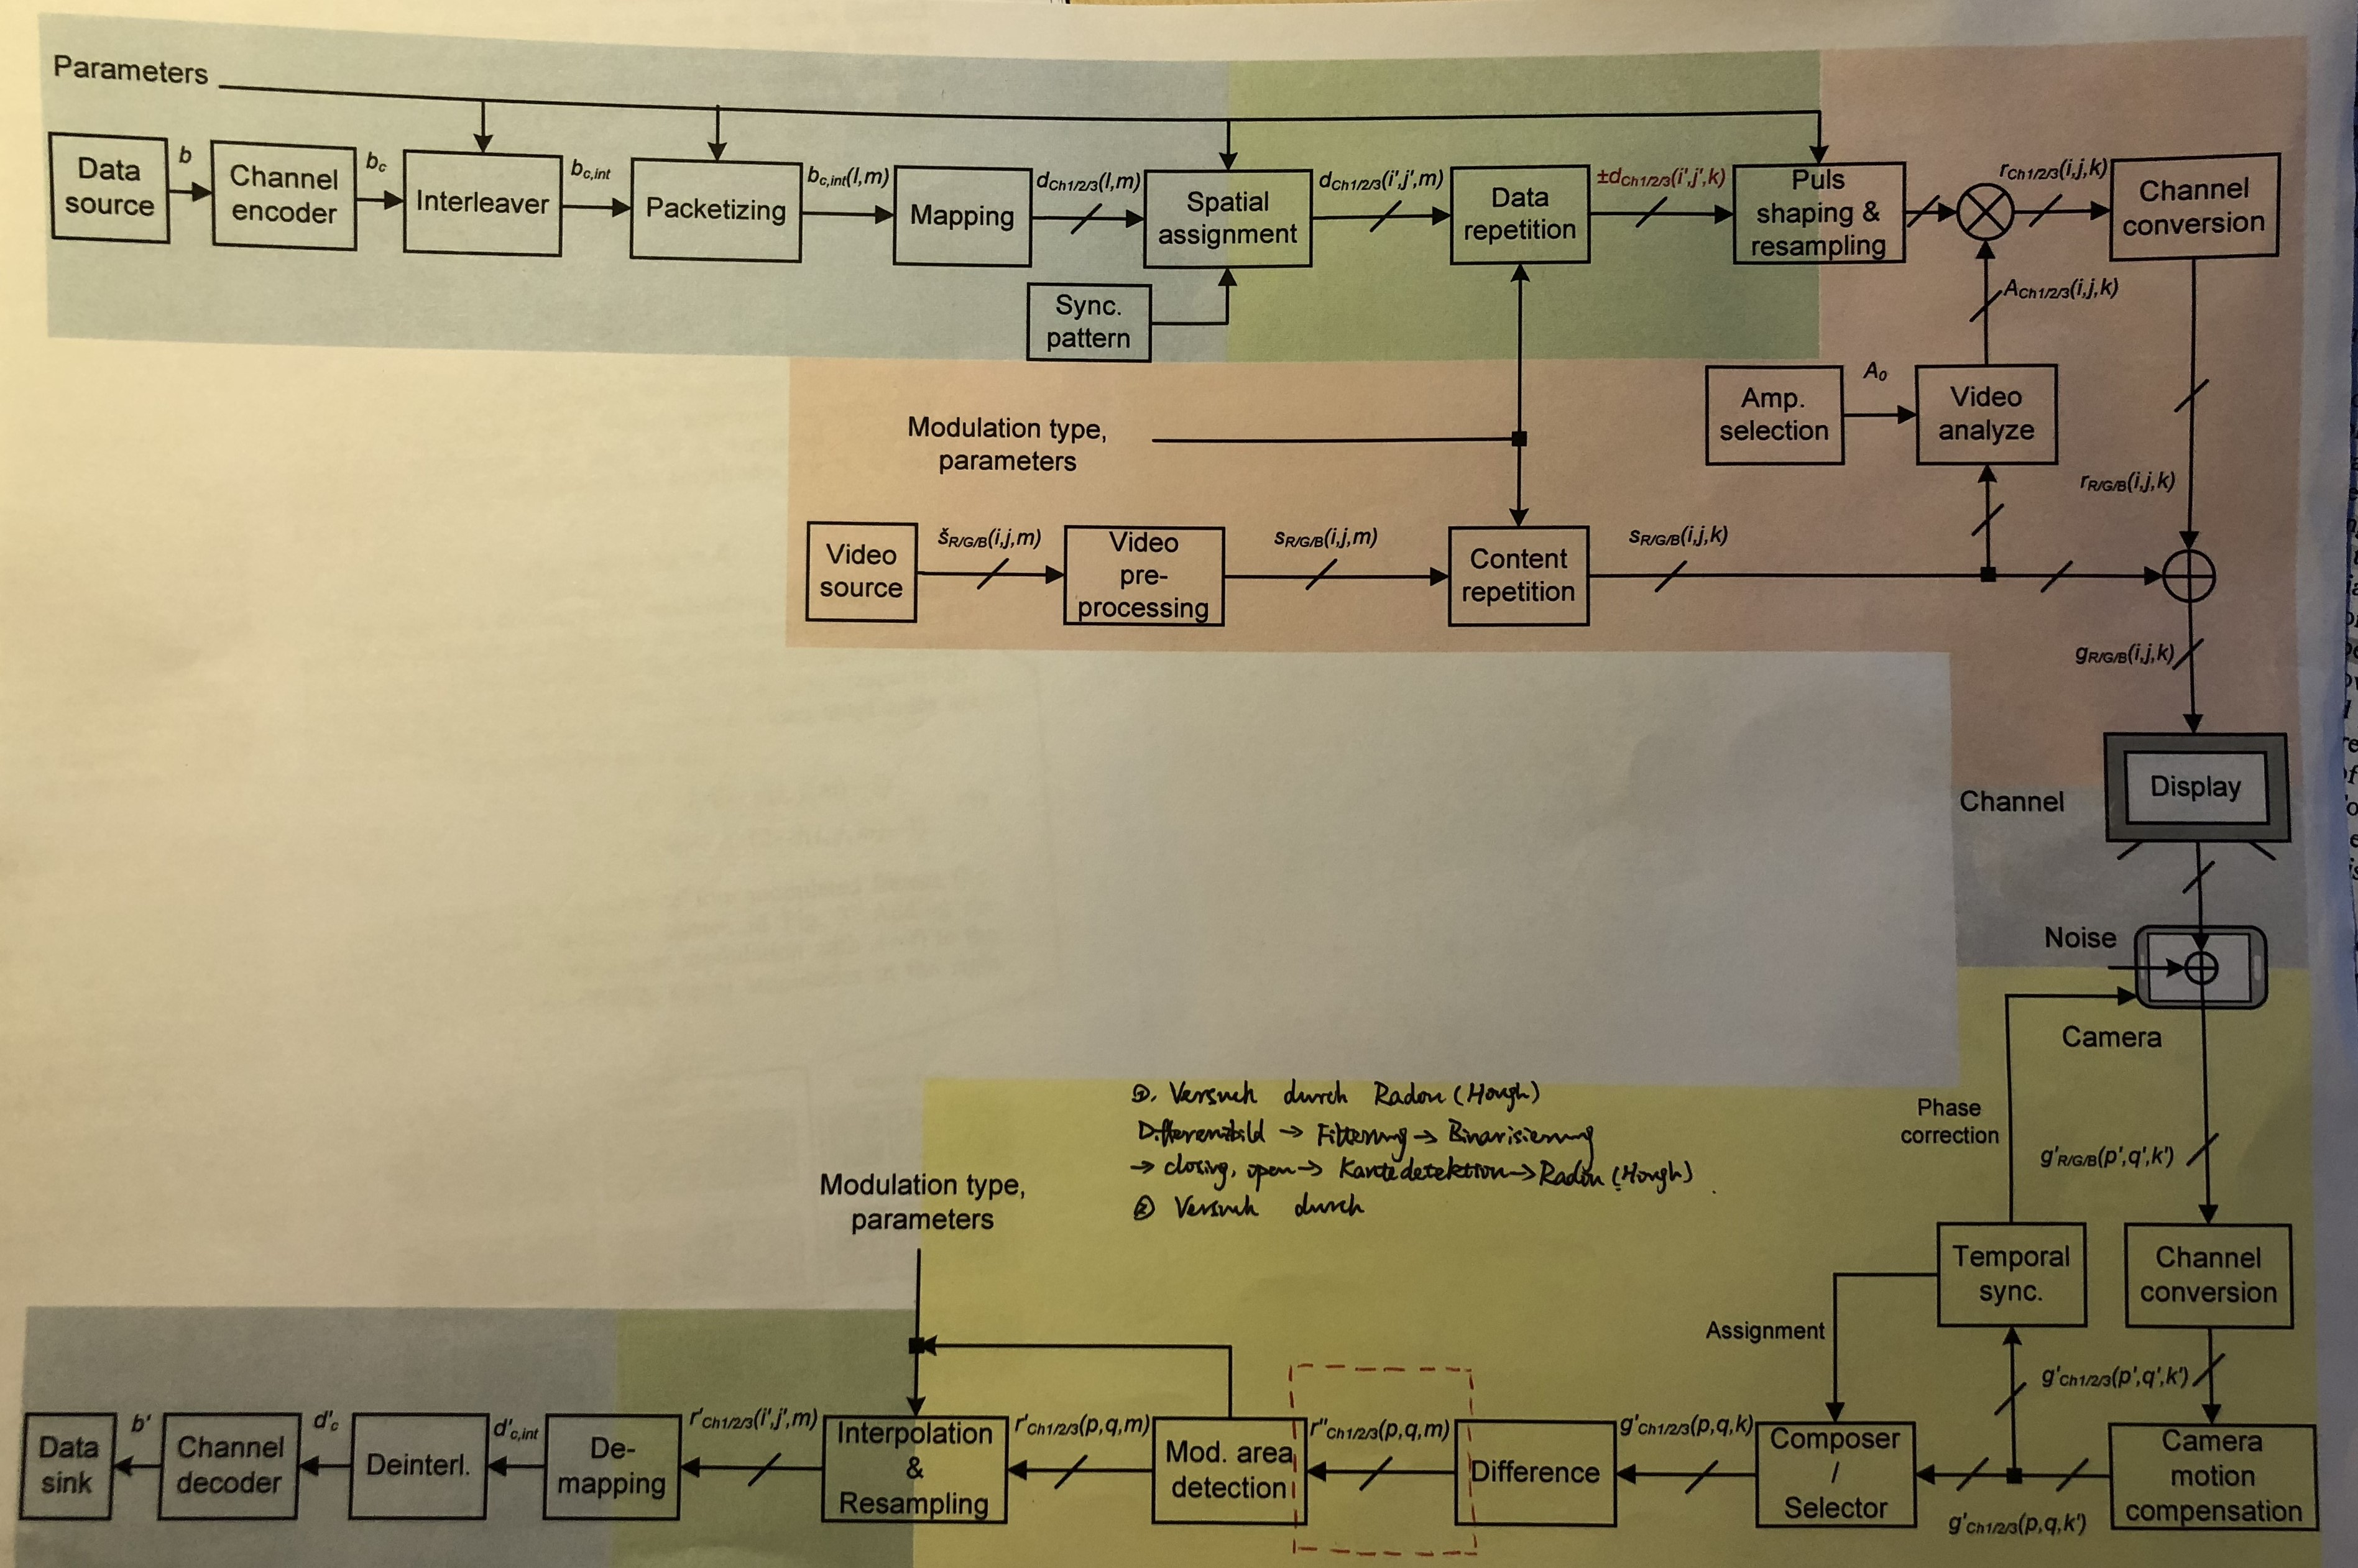
\includegraphics[keepaspectratio,width=1.0\textwidth]{images/David3.jpg}
	\caption{Schematische Darstellung von DaVid System}
	\label{fig:David2}
\end{figure}


\subsection{Modulationsverfahren}

Ein Modulationsverfahren, das die Videoqualität nicht offensichtlich reduziert garantiert, ist sehr wichtig für ein auf Videogerät basierendes Datenübertragungssystem. Die möglichen Modulationsverfahren in DaVid-System sind:
\begin{itemize}
	\item Zeitliche differentielle Modulation der Luminanz
	\item Zeitliche differentielle Modulation der Chrominanz
	\item Örtliche differentielle Modulation der Luminanz
	\item Örtliche differentielle Modulation der Chrominanz
\end{itemize}

Zeitliche differentielle Modulationsverfahre lässt kontinuierliches Paar Frames den gleichen Luminanz- bzw. Chrominanz-Videoinhalt enthalten, d.h. durch Subtrahieren die mit daten addiert Kanal der Paar Frames die Differenzbild erhalten lassen können. Dagegen in örtliche- sind die benachbarte Pixel mit den gleichen Videoamplituden. Im Vergleich zu Luminanzteil Y die Anzeigequalität in U und V Komponente ist signifikant besser, wenn Informationen in Chrominanz wiederholt und moduliert werden. Deswegen wird in dieser Arbeit nur zeitliche differentielle Modulation der Chrominanz verwendet. Abbildung 2.3 zeigt ein Blockdiagramm einer typischen Senderimplementierung durch zeitliche differentielle Modulation.

\begin{figure}[htb]
	\centering 
	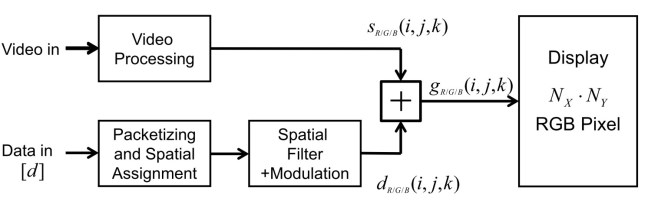
\includegraphics[keepaspectratio,width=0.8\textwidth]{images/David2.jpg}
	\caption{Blockschaltbild der Signalverarbeitung in zeitlicher differentieller Modulation}
	\label{fig:David3}
\end{figure}

Wir nehmen eine Diaplay an, die in horizontale Richtung $N_x$ Pixel stehen, dagegen in vertikale Richtung $N_y$ Pixel. Das Videoeingangssignal wird verarbeitet, um eine Anzeigeeingabe $s(i,j,k)$ zu liefern. Mit zeitliche differenziell Modulation ist die Videoinhalt des kommenden Frame dasselbe.Die Indizes i und j bedeuten die horizontale und vertikale Pixelposition auf dem Bildschirm, während k die Nummer des reproduzierten Bildes ist.
Indiz m heißt den Zähler des Frames in einer Videosequenz. Der Amplitudenbereich des Videosignals sollte begrenzt sein, um die Addition kleiner Datenamplituden ohne Übersteuern zu ermöglichen.

\begin{equation}
\begin{split}
 s_{R/G/B}&(i,j,k+1) = s(i,j,k) \\
          &  for \ 0\le i <N_x, 0\le j<N_y,k=2 \cdot m , m \in \mathbb{Z}\\
\end{split}
\end{equation}

Vor Datenübertragung muss der Datenstrom in Schichten der Länge L aufgeteilt werden. Indiz L bedeutet die Menge der Daten, die in einem Framepaar übertragen werden können. Ein direkter Ansatz ist eine direkte Zuordnung von Datenbits zu Pixeltripeln Zeile für Zeile.

\begin{equation}
\begin{split}
  & d(l)\rightarrow d(i,j,m) \qquad d(l)\in \{-1,1\} \\
  & 0\le l <L,L = N_x \cdot N_y \\
  & i=l \bmod N_x \qquad j=\lfloor l/N_x \rfloor \\
\end{split}
\end{equation}

Die Modulationsamplitude A ist ein wichtiger Parameter für Datenübertragung. Im Prinzip kann die Amplitude in verschieden Kanal unabhängig gewählt werden, um die Systemleistung zu optimieren. In diesen Arbeiten setzen die Amplitude gleichwertig.

\begin{equation}
 A_R=A_G=A_B=A        
\end{equation}

Das differentielle Modulationsverfahren ordnet jede Sequenz von $\left\{-A, A\right\}$ zu d = -1 bzw. $\left\{A, -A\right\}$ zu d = 1 zu. Modulierte Datensymbole und verarbeitete Videoamplituden werden addiert, um die Anzeigeeingabe $g(i,j,k)$ zu liefern:

\begin{equation}
\begin{split}
   s_{R/G/B}(i,j,k)  &= s_{R/G/B}(i,j,m) + A_{R/G/B} \cdot \left( 2 \cdot d(i,j,m) - 1 \right) \\
   s_{R/G/B}(i,j,k+1)&= s_{R/G/B}(i,j,m) - A_{R/G/B} \cdot \left( 2 \cdot d(i,j,m) - 1 \right) \\
\end{split}
\end{equation}

Ein Beispiel einer modulierten Bildfolge ist in Abbildung 2.4 gezeigt. Das Hinzufügen der modulierten Daten (hier mit A = 4) zu dem Videoeingang ergibt die Anzeigeamplituden in der rechten Spalte.
\newpage

\begin{figure}[htb]
	\centering 
	\includegraphics[keepaspectratio,width=0.8\textwidth]{images/David4.jpg}
	\caption{Ein Beispiel einer modulierten Bildfolge}
	\label{fig:David4}
\end{figure}



\subsection{DatenBlock}

Um die Anforderungen an die Kameraauflösung zu lockern, Ein einfaches und unkompliziertes Verfahren ist Zuordnung jedes Datenbits zu einem Block von $B_X \times B_Y$ Pixeln.

\begin{equation}
\begin{split}
  & d(l)\rightarrow d(x,y,k) \qquad 0\le l <L \\
  & L=\lfloor N_X/B_X \rfloor \cdot \lfloor N_Y/B_Y \rfloor \\
  & x=(l \cdot B_X) \bmod N_X +r_X, \ r_X =0...(B_X -1) \\
  & y=\lfloor l / \lfloor N_X/B_X \rfloor \rfloor \cdot B_Y +r_Y, \ r_Y =0...(B_Y -1) \\
\end{split}
\end{equation}

Wenn die Anzahl der Pixel pro Zeile kein Vielfaches von $B_X$ ist oder wenn die Anzahl der Pixel kein Vielfaches von $B_Y$ ist, muss die Anzahl der Pixel und Zeilen, die für die Modulation in Gleichung $\left(2.5\right)$ verwendet werden, ersetzt werden durch:

\begin{equation}
\begin{split}
  & N_X = \lfloor N_X/B_X \rfloor \cdot B_X\\ 
  & N_Y = \lfloor N_Y/B_Y \rfloor \cdot B_Y\\ 
\end{split}
\end{equation}

\newpage
In dieser Arbeit werden das DatenBlock für quadratische Blöcke gesetzt.

\begin{equation}
   B_X = B_Y = B.
\end{equation}





\section{Anwendungsgebiete} 
%\label{sec:Anwendungsbereiche}

Die Datenübertragungsrate des David-Systems wird voraussichtlich erreicht bis zu 100 Mbit/s. Es gehöre	zu einer Sichtlinienübertragung für kurze Verbindungen. Geeignete Abdeckungsbereichen hängen von der Größe des Displays und der Kameraoptik ab. Obwohl im Vergleich zum letzten WLAN- Versionen \gls{ieee} 802.11, die Leistung scheint nicht so attraktiv. Der Vorteil liegt nicht nur in der wachsenden Leistungsfähigkeit von Video-Display und Kamera, aber auch die Option zur Wiederverwendung der bestehenden Hardware, die zum Zeigen des Videos installiert wurde. Ein empfohlene praktische Anwendungsbereich des DaVids ist öffentlicher Ort, z.B. U-Bahn-Station, großes Stadion und so weiter. Annehmen eine Situation, wenn die Leute auf ihre U-Bahn warten, sie können ihre eigene Software aktualisieren, indem Sie einfach auf die zeigende Werbung in dem Bildschirm leiten.

Berücksichtigen der Eigenschaften des DaVids, d.h. die Synchronisation von Videospielen und Datenübertragung. Viele Anwendungsszenarien können in Betracht gezogen werden und scheinen sehr attraktiv zu sein. Die drei Hauptszenarien sind:

\begin{itemize}
  \item Indoor-individuelle Kommunikation: Kurzstreckenverbindungen basieren auf relativ kleinen (Tablet-Größe) Bildschirm, Anwendungen z.B. die Übertragung von Hintergrundinformationen an Besucher im Museum, Kiosk.
  \item Indoor-Multicast-Kommunikation:Streckabstand ist länger als ersten Fall auf relativ größer (40-100") Bildschirm, Anwendungen z.B. während Videoabspielen Besucher die Anwendungsdaten oder Mediendateien herunterladen können im Kiosk, Restaurant.
  \item Freien Kommunikation: Größter Bildschirm wie im Einkaufszentren oder Sport-Arenen, Anwendungen können denen des zweiten Szenarios ähneln.
\end{itemize}

Sobald die Dienste auf öffentlichen Bildschirmen implementiert werden, kann Leute mit Hilfe eines modernen Smartphones, die mit einer geeigneten Kamera eingebaut ist, nach der Installation einer neuen App innovative wahrnehmen.





















